\documentclass[12pt]{article}
\usepackage{../thesis_style}

\title{Chapter 4: Fredholm problem of wave operator on torus}
\date{}

\begin{document}
\maketitle
In previous chapter, we have shown that any (globally) elliptic pseudodifferential operator $A \in \Psi^{m}_{\infty}(\R^n)$ give raise to a Fredholm operator between the Sobolev spaces
\begin{align*}
A : H^s \to H^{s - m}. 
\end{align*}
Presently, we shall turn our focus to to a simple non-elliptic problem. Specifically, we will consider the Fredholm problem of the wave operator on the torus. We shall first give the definitions of the manifolds and Hilbert spaces that will feature in this problem. \\

\begin{fdefinition} 
Let $\S^1 = [0,1] / (0 \sim 1)$ denote the circle and for any $k \in \N$ let
\begin{align*}
\T^k := \underbrace{\S^1 \times \S^1 \times \dots \times \S^1}_{k}
\end{align*}
denote the $k$-dimensional torus. We shall study the totally periodic wave operator, on $M :=  = \T_t^1 \times \T_x^{n}$ given by
\begin{align}\label{eq: d'Alembertian}
\Box := \p_t^2 - \sum_{j = 1}^{n -1} \p_{x_j}^2
\end{align}
where $(t, x_1, \dots, x_n)$ are the local coordinates on $M$. 
\end{fdefinition}
Note first that $\Box$ is a second order differential (and thus pseudodifferential) operator with \textit{homogeneous} principal symbol given by 
\begin{align*}
\sigma_2(\Box)(t, x, \tau, \xi) = \xi_1^2 + \xi_2^2 + \dots + \xi_{n}^2 - \tau^2 = \abs{\xi}^2 - \tau^2. 
\end{align*}
Thus, the characteristic set is given by the zero set of the principal symbol (excluding the zero section), i.e. 
\begin{align*}
\Char^2(\Box) = \set{\sigma_2(\Box) = 0} \setminus \set{(t, x, \tau, \xi) \wh \tau = \xi = 0}
\end{align*}
which lies precisely on the `light cone' emanated from every point $(t, x) \in M$, i.e.  
\begin{align*}
\Char^2(\Box) := \set{(t, x, \tau, \xi) \wh 0 \neq \abs{\xi}  = \abs{\tau}} 
\end{align*} 

So, clearly the operator is not elliptic everywhere. However, using the results we have accumulated thus far and a further result described below, we shall show that we can perturb the wave operator by a ``complex absorbing potential" \ref{}, $iQ$ so that $\Box - iQ$ is a Fredholm operator as a map 
\begin{align*}
\Box - iQ : \mathcal{X}^s \to H^{s -1}(M)
\end{align*}
where $\mathcal{X}^s$ is a non-trivial subspace of $H^s(M)$. This will be the goal of this chapter. 



\paragraph{Strategy of the proof} \hfill \\
The crucial step in the proof is to show that the following \textit{Fredholm estimates} holds: $\forall s, N \in \R$, $\forall u \in \mathcal{X}^s$, there exist positive real number $C > 0$, such that
\begin{align*}
&\norm[u]_{H^s} \leq C \brac{ \norm[(\Box - i Q)u]_{H^{s - 1}} + \norm[u]_{H^N}} \\
&\norm[u]_{H^s} \leq C \brac{ \norm[(\Box + i Q^*)u]_{H^{s - 1}} + \norm[u]_{H^N}}. 
\end{align*}
First, we note that in the elliptic set $\Ell^2(\Box)$, microlocal elliptic regularity estimate \ref{} provide us with sharper estimates. However, to obtain the estimates above near elements in the characteristic set $\Char^2(\Box)$, we will need to ``propagate" results from elliptic regions along the Hamiltonian flow of $p = \sigma_2(\Box)$. This is where we will employ propagation of singularity theorem described in the next section. Indeed, this method will prompt us to construct $Q$ to introduce a larger region in $T^*M$ where $\Box - iQ$ is elliptic, so that every point in the characteristic set of $\Box - iQ$ is a point along the Hamiltonian flow that begins in $\Ell^2(\Box - iQ)$. 



\paragraph{Significance} \hfill \\
One characterisation of Fredholm operators is that they are operators that are invertible up to a compact operator. Moreover, our result will allow us conclude the regularity of the solutions to differential equation of the form 
\begin{align*}
(\Box - iQ) u = f, \quad u, f \in H^{-\infty}(M)
\end{align*}
in terms of the regularity of $f$. One immediate consequence of the estimates given above is that if $f$ is smooth, we know that $\norm[(\Box - iQ)u ]_{H^{s-1}}$ (i.e. right hand side of estimate) is bounded for all $s \in \R$ and therefore $\norm[u]_{H^s}$ (left hand side) is bounded for all $s \in \R$. In short, we have the result 
\begin{align*}
f \in C^\infty(M) \iff u \in C^\infty(M). 
\end{align*}
In particular, solutions to the homogeneous equation $(\Box - iQ)u = 0$ is guarantee to be smooth. \\


Furthermore, the method we shall employ relies only on the \emph{principal symbol} of $\Box$ which is second order. This allows us to extend the result to any first order pertubation, i.e. any choice of $A \in \Psi^{1}_{\infty}(\R^n)$ give rise to a continuous (in fact, analytic) operator valued map 
\begin{align*}
f : z \mapsto (\Box - iQ + zA)
\end{align*}
where $f(z) : \mathcal{X}^s \to H^{s - 1}(M)$ is Fredhom any $z \in \C$. Recall that the Fredholm index defined by
\begin{align*}
\mathrm{Ind}(T) := \dim \ker T - \dim \coker T, \quad T \text{ Fredholm }
\end{align*}
is a continuous as a map from the space of Fredholm maps between Hilbert spaces to $\Z$ \ref{}. 
\todo{something about constant index} 




\section{Propagation of singularities} 

\subsection{A motivation example} 
To motivate this result, we will first look at the example of the wave operator in $2D$ Euclidean space, i.e. the operator
\begin{align*}
\p_t^2 - \p_x^2. 
\end{align*}
Using the factorisation $(\p_t^2 - \p_x^2) = (\p_t + \p_x) (\p_t - \p_x)$, we can easily obtain the solution to the homogeneous differential equation 
\begin{align}
(\p_t^2 - \p_x^2) u = 0 \iff u(t, x) = g(x -t) + h(x + t) \label{eq: homogeneous wave in 1d} 
\end{align}
where $g, h$ are continuous functions defining the right and left moving waves respectively. Notice that if $g(x)$ is not differentiable at $x_0 \in \R$, then $u(t, x)$ is not differentiable on the light cone $\set{x - t = x_0}$ emanated from the initial point $(t, x) = (0, x_0)$. Similarly, any initial singularity $x_1 \in \R$ of $h$, will be propagated to points on the light cone $\set{x + t = x_1}$. 

\begin{center}
    \begin{tikzpicture}
    \draw[->] (0, 3) -- (6, 3);
    \node at (6.2, -0.2) {$x$}; 
    \draw[->, thick] (0, 0) -- (0, 6);
    \node at (-0.2, 6.2) {$t$};  
    
    \node at (3, 2.6 ) {$x_0$}; 
    \draw (3, 2.9) -- (3, 3.1); 
    
    
    \draw [->] (1, 1) -- (5, 5); \node at (5.5, 5.5) {$\set{x - t = x_0}$}; 
    \draw [<-] (1, 5) -- (5, 1); \node at (1.5, 5.5) {$\set{x + t = x_0}$}; 
    \end{tikzpicture}
\end{center}

Thus, we can conjecture that for any solution $u$ to the homogeneous equation \ref{eq: homogeneous wave in 1d}, either $u(t, x)$ is differentiable at $(t_0, x_0)$, or the same singular behaviour (i.e. non-differentiability) will be present on all of the light cone 
$$\set{(t_0 + s, x_0 +s) \wh s \in \R} \cup \set{(t_0 - s, x_0 + s) \wh s \in \R}.$$

 We shall see that this phenomenon generalise to arbitrary manifolds, with ``light cone" replaced by the bicharacteristic flow of the principal symbol of the operator under investigation. 

\todo{example on euclidean wave operator in one space dimension}
\todo{insert discussion + proof sketch of prop of sing theorem}

\begin{ftheorem}[Propagation of singularities] 
    Suppose we have 
    \begin{enumerate}
        \item $P \in \Psi^k_{cl}(\R^n)$ a properly supported operator,
        \item $\sigma_{k}(P) = p - iq$ for real polyhomogeneous symbols $p, q \in S^{k}_{ph}(\R^{2n}; \R^{n})$, 
        \item $A, B, B' \in \Psi^{0}_{cl}(\R^n)$ compactly supported and $q \geq 0 $ on $\WF(B')$, 
        \item for all $(x, \xi) \in \WF(A)$, there exists $\sigma \geq 0$ such that for all $t \in [-\sigma, 0]$
        \begin{align*}
            \exp(-t\sym[\xi]^{1-k}H_p)(x, \xi) \in \Ell(B)
        \end{align*}
    \end{enumerate}
    then for all $s, N \in \R$ and $u \in C^\infty(\R^n)$, there exist $C > 0$ such that 
    \begin{align*}
        \norm[Au]_{H^s} \leq C\brac{\norm[Bu]_{H^s} + \norm[B'Pu]_{H^{s - k + 1}} + \norm[u]_{H^{-N}}}. 
    \end{align*}
\end{ftheorem}



\section{Fredholm problem of totally periodic wave operator} 
We will now define the required operator $Q$ and the subspace $\mathcal{X}^s \subset H^{s}(M)$ that make $\Box - iQ: \mathcal{X}^s \to H^{s -1}$ Fredholm.  As mentioned we will proceed via the ``complex absorption" method \ref{}. We define
\begin{align*}
Q := \chi(t)^2 \p_t^2
\end{align*}
where $\chi : \S^1 \to [0, 1]$ is a smooth cut-off satisfying
\begin{align*}
\chi(t) = 
\begin{cases}
1 & t \geq  1 - \delta \text{ or } t \leq \delta \\
0 &  \delta + \delta' < t < 1 - \delta - \delta'
\end{cases}
\end{align*}
where $\delta, \delta' \in (0, 1/8)$ (ensuring that $\delta+ \delta' < 1/4$). 

\begin{center}
    \begin{tikzpicture}
    \draw [] (0, 0) rectangle (8, 8);
    \draw[pattern=north west lines, pattern color=blue, opacity=0.5] (0, 0) rectangle (8, 2.5);
    \draw[pattern=north west lines, pattern color=blue, opacity=0.5] (0, 5.5) rectangle (8, 8);
    
    \draw[pattern=north east lines, pattern color=red, opacity=0.5] (0, 2.25) rectangle (8, 5.75); 
    \draw [thick] (0, 2.25) -- (8, 2.25); 
    \draw [thick] (0, 5.75) -- (8, 5.75); 
    
    \draw  [dashed] (-2.5, 2) -- (8.1, 2);
    \draw  [dashed] (-2.5, 6) -- (8.1, 6);
    \draw  (-0.5, 5.5) -- (8.1, 5.5);
    \draw  (-0.5, 2.5) -- (8.1, 2.5);
    \node at (8.6, 2) {$\delta$}; 
    \node at (8.6, 6) {$1 - \delta$};
    \node at (8.7, 2.5) {$\delta + \delta'$}; 
    \node at (9, 5.5) {$1 - \delta - \delta'$};

    
    \node at (8.3, -0.1) {$x$};
    \node at (-0.1, 8.3) {$t$}; 
    \node at (-0.2, -0.2) {$0$};
    \node [fill=white]  at (4, 7) {$U_1 :=  \set{\chi(t) \neq 0}$ };
    \node [fill=white] at (4, 1) {$U_1$};
    \node [fill=white] at (4, 4) {$U_2 = $ a neighbourhood of $\set{\chi(t) = 0}$};
    
    
    \draw [->, thick] (-0.5, 0) -- (-3, 0); 
    \draw [->, thick] (-0.5, 0) -- (-0.5, 8);
    \draw [-, thick] (-2.5, 0.1) -- (-2.5, -0.1);
    \node at (-3.3, -0.3) {$\chi(t)$};
    \node at (-2.5, -0.3) {1}; 
    
    \draw (-2.5, 0) -- (-2.5, 2);
    \draw[rounded corners=8pt] (-2.5, 2) -- (-2.5, 2.24) -- (-1, 2.25) -- (-0.5, 2.5);
    \node at (-2.5, 8) (right start) {};
    
    \draw (-2.5, 8) -- (-2.5, 8 - 2);
    \draw[rounded corners=8pt] (-2.5, 8 - 2) -- (-2.5, 8 - 2.24) -- (-1, 8 - 2.25) -- (-0.5, 8 - 2.5);
    \end{tikzpicture}
\end{center}
We note that $\Box - iQ$ is again a second order differential operator, but its principal symbol changes to 
\begin{align}
\sigma_2(\Box - iQ)(t, x, \tau, \xi) = \abs{\xi}^2 - \tau^2 + i \chi(t) \tau^2 \label{eq: p - iq} 
\end{align}
which, like $\sigma_2(\Box)$, remains homogeneous to second degree in the dual variables, $(\tau, \xi)$. The characteristic set of $\Box - iQ$ is given by the zero set of (\ref{eq: p - iq}) minus the 0 section. In $U_2$, where $\chi(t) = 0$: 
\begin{align*}
\sigma_2(\Box - iQ) = 0 \iff \abs{\xi} = \abs{\tau}. 
\end{align*} 
On the other hand, outside of $U_2$, $\chi(t) \neq 0 $. Thus, the imaginary part of $\sigma_2(\Box - iQ)$ is zero only if $\tau = 0$ which implies that $\xi = 0$ if the real part were to be zero as well. Thus, $\sigma_2(\Box - iQ) = 0$ in $U_2^c$ only if $\xi = \tau = 0$ which is the zero section excluded from the characteristic set. In short, the characteristic set is given by the close set 
\begin{align*}
\Char^2(\Box - iQ) 
& = \set{\sigma_2(\Box - iQ) = 0} \setminus 0 \\
& = \set{(t, x, \tau, \xi) \wh \chi(t) \neq 0 \text{ and }  0 \neq \abs{\xi} = \abs{\tau}} \subset T^* M \setminus 0. 
\end{align*}

We see now that the pertubation $Q$ introduced a region, $T^*U_1 \subset T^*M$, called the absorption region where $\Box - iQ$ is (microlocally) elliptic. 

\todo{Mention the sympletic structure on the torus and the Hamiltonian flow $\exp(sH_p)(t, x, \tau, \xi) = (t + s\tau, x + s \xi, \tau, \xi)$. As expected, this is tangential to the characteristic set.}

The estimate provided by the propagation of singularity theorem suggest that we give the following definition for $\mathcal{X}^s$. 

\begin{fdefinition}
    Let $M$ be the manifold and $\Box -i Q$ be the operator defined above \ref{}. For each $s \in \R$, we define a subspace of $H^{s}(M)$ given by
    \begin{align*}
    \mathcal{X}^s = \set{u \in H^s(M) \wh (\Box - i Q)u \in H^{s - 1}(M)}. 
    \end{align*}
    Note that $\mathcal{X}^s$ is a Hilbert space (see lemma \ref{}) with inner product and associated norm given by 
    \begin{align*}
    &\inprod[u, v]_{\mathcal{X}^s} := \inprod[u, v]_{H^{s}} + \inprod[(\Box - iQ)u, (\Box - iQ)v]_{H^{s -1}} \\
    & \norm[u]_{\mathcal{X}^s}^2 = \inprod[u, u]_{\mathcal{X}^s} = \norm[u]_{H^s}^2 + \norm[(\Box - iQ)u]_{H^{s - 1}}^2
    \end{align*}
    for all $u, v \in \mathcal{X}^s$. 
\end{fdefinition}

\begin{flemma}
    Let $A_j \in \Psi^{m_j}_{\infty}(M)$ and $s_j \in \R$ for $j \in \set{1, \dots, N}$. Define the linear subspace of $H^{s}(M)$ by 
    \begin{align*}
    \mathcal{X} := \set{u \in H^{s} \wh A_ju \in H^{s_j}, j = 1, \dots, N},
    \end{align*}
    then with the norm
    \begin{align*}
    \norm[u]_{\mathcal{X}}^2 := \norm[u]_{H^s}^2 + \sum_{j = 1}^N \norm[A_j u]_{H^{s_j}}^2
    \end{align*}
    $\mathcal{X}$ is complete. 
\end{flemma}
\begin{proof}
    Let $\set{u_k}_{k=1}^\infty $ be a Cauchy sequence in $\mathcal{X}$, i.e. for any $\epsilon > 0$
    \begin{align*}
    \norm[u_k]_{H^s}^2 + \sum_{j = 1}^N \norm[A_j u_k]_{H^{s_j}}^2 < \epsilon
    \end{align*}
    which in turn implies that each $A_ju_k \in H^{s_j}$ are Cauchy. By completeness of $H^s$ and $H^{s_j}, j = 1, \dots, N$, we get $v$ and $v_j$'s such that 
    \begin{align*}
    &u_k \to v \in H^s\\
    &A_j u_k \to v_j \in H^{s_j}. 
    \end{align*}
    Then, by continuity of $A_j : H^s \to H^{s - m_j}$, we have 
    \begin{align*}
    v_j = \lim_{k \to \infty} A_j u_k = A_j \lim_{k \to \infty}u_k = A_j v. 
    \end{align*}
    Since $v_j \in H^{s_j}$, the equality above gives $A_jv \in H^{s_j}$ for each $j = 1, \dots, N$. Therefore, $v \in \mathcal{X}$. Furthurmore, for any $\epsilon > 0$, the convergence in $H^s$ and $H^{s_j}$ above give the bounds that $ \norm[u_k - v]_{H^s}^2 < \epsilon / (N + 1)$ and $\norm[A_j u_k - v_j]_{H^{s_j}}^2 < \epsilon / (N +1)$ for large enough $k \in \N$. Therefore, 
    \begin{align*}
    \norm[u_k - v]_{\mathcal{X}} 
    &= \norm[u_k - v]_{H^s}^2 + \sum_{j = 1}^N \norm[A_j u_k - A_jv]_{H^{s_j}}^2\\
    &= \norm[u_k - v]_{H^s}^2 + \sum_{j = 1}^N \norm[A_j u_k - v_j]_{H^{s_j}}^2 \\
    & < (N + 1) \cdot \frac{\epsilon}{N + 1} \\
    & = \epsilon. 
    \end{align*}
    Hence, every $\mathcal{X}$-Cauchy sequence converges in $\mathcal{X}$ as required. 
    
\end{proof}



With the definitions, in place, we are ready to prove: 
\begin{ftheorem}
    For each $s \in \R$, the operator
    \begin{align*}
    (\Box - iQ): \mathcal{X}^s \to H^{s - 1}(\T^n)
    \end{align*}
    is Fredholm. 
\end{ftheorem}
\begin{proof}
    As mentioned, we need to show that $\forall s, N \in \R$, $\forall u \in \mathcal{X}^s$, there exist positive real number $C > 0$, such that
    \begin{align} \label{eq : fredholm estimate for wave operator} 
    &\norm[u]_{H^s} \leq C \brac{ \norm[(\Box - i Q)u]_{H^{s - 1}} + \norm[u]_{H^N}} \\
    &\norm[u]_{H^s} \leq C \brac{ \norm[(\Box + i Q^*)u]_{H^{s - 1}} + \norm[u]_{H^N}}. 
    \end{align}
    Since the estimates above will be proven for all $s \in \R$, adding the term involving $H^{s-1}$-norm on both sides and recalling that the dual of Sobolev spaces are given by $(H^{s - 1})^* = H^{1 - s}$the estimates above translate to : $\exists C > 0$, 
    \begin{align*}
    \norm[u]_{\mathcal{X}^s} = \norm[u]_{H^s} + \norm[(\Box - iQ)u]_{H^{s - 1}} \leq C \brac{ \norm[(\Box - i Q)u]_{H^{s - 1}} + \norm[u]_{H^N}}
    \end{align*}
    Also, since the torus $M$ is a compact manifold, $H^{r}(M) \hookrightarrow H^{r'}(M)$ is a compact inclusion for any $r' < r$. Thus, by \ref{}, $\Box - iQ$ has finite dimensional kernel and closed range. Furthermore, by \ref{} and the observation that $(\Box - iQ)^* = \Box^* + iQ^* = \Box + iQ^*$, we have
    \begin{align*}
    \coker (\Box - iQ) \cong \ker(\Box + iQ^*). 
    \end{align*}
    But again by \ref{} and the second estimate, we conclude that $\ker (\Box + iQ^*)$, and hence $\coker (\Box - iQ)$, is finite dimensional. Jointly, these allow us to conclude that $\Box - iQ : \mathcal{X}^s \to H^{s - 1}(M)$ is Fredholm. \\
    
%    Note that $(\Box - iQ)^* = \Box + i Q^*$. Also, since $M$ is a compact manifold, \ref{} shows that $H^{s} \hookrightarrow H^{N}$ is a compact inclusion for $N < s$. \todo{proof that this transfer to $\mathcal{X}^s$ as well}. Then, by \ref{}, these esitmates allow us to conclude that $(\Box - iQ) : \mathcal{X}^s \to H^{s - 1}$ is indeed a Fredhold operator.     \\
%    \\
    It remains to prove the aforementioned Fredholm estimates. Let $s, N \in \R$, $u \in \mathcal{X}^s$ be given. First, we will establish a sharper estimate in the absorption region where $\Box - iQ$ is elliptic. Let $\chi_1 \in C^{\infty}_c(T^*M)$ be a smooth compactly supported cut-off with $\supp \chi_1 \subset U_1 \subset \Ell^2( \Box - iQ)$. Explicitly, we can choose
    \begin{align*}
    \chi_1(t, x, \tau, \xi) = \chi(2 t), \quad \supp(\chi_1) \subset \set{\chi(2t) \neq 0} \subset \set{\chi(t) \neq 0} = U_1
    \end{align*}
    We note that multiplication by $\chi_1$ act as a $0^{th}$ order pseudodifferential operator. Its wavefront set are points where it is non-zero, i.e. 
    \begin{align*}
    \WF'(\chi_1) = \set{(t, x, \tau, \xi) \wh \chi(2t) \neq 0 } \subset \Ell^2(\Box - iQ)
    \end{align*}
    and thus microlocal elliptic regularity estimate applies to give \todo{remember to include Vasy's microlocal estimate} \ref{} : $\exists C > 0$ such that
    \begin{align*}
    \norm[\chi_1 u]_{H^s} \leq C \brac{\norm[(\Box - iQ)u ]_{H^{s - 2}} + \norm[u]_{H^N}}
    \end{align*}
    
     Outside the absorption region, however, we will rely on propagation of singularity estimate. The crucial geometric observation is that every light ray eminating from a point in $U_1^c$ can be traced, in both forward and backward direction, to a source in $U_1$. In other words, every element of $\Char^2(\Box - iQ)$ outside of the absorption region lies along the Hamiltonian flow of the principal symbol of $\Box$ that begins in the absorption region. In symbols,  
     \begin{align*}
     &(t, x, \tau, \xi) \in \Char^2(\Box - iQ) \\
     \iff & \chi(t) = 0 \text{ and } \abs{\tau} = \abs{\xi}\\
     \iff & \exists (t', x', \tau', \xi') = (t', x', \tau, \xi) \in \Ell^0(\chi_1), \\
      & \exp(\sigma H_p)(t', x', \tau', \xi') = (t' + \sigma t, x + \sigma \xi, \tau, \xi) = (t, x, \tau, \xi)
     \end{align*}
     for some $\sigma  \in \R$. We have use the fact that $\Ell^0(\chi_1) = \set{\chi_1 \neq 0 } \subset U_1$. In fact, we can always choose $t' = 0$, since the light ray eminating from the line $t' = 0$ will cover every  
     
     
     \begin{center}
         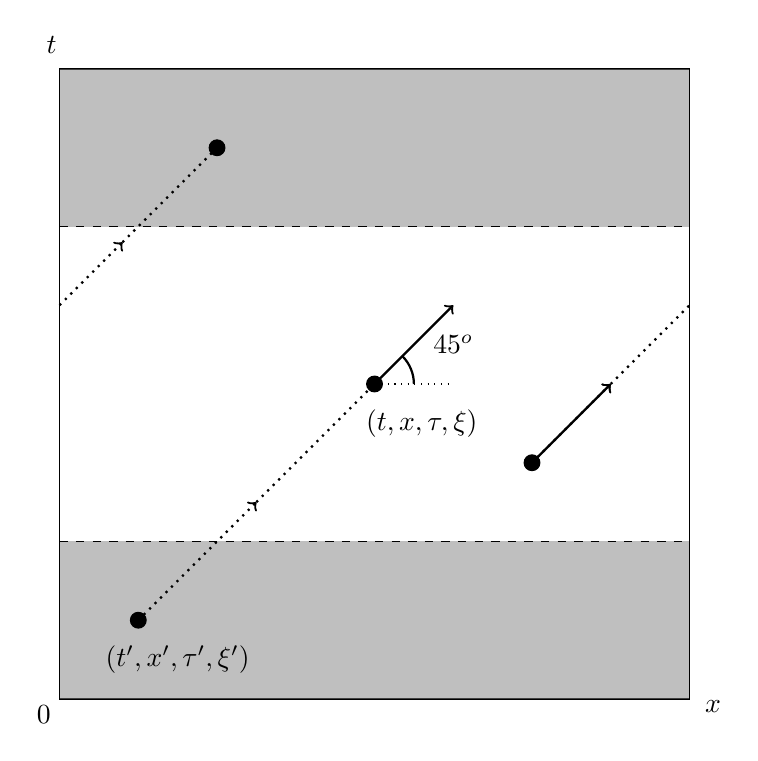
\begin{tikzpicture}
         \draw [] (0, 0) rectangle (8, 8);
         \fill [gray, opacity=0.5] (0, 0) rectangle (8, 2);
         \fill [gray, opacity=0.5] (0, 6) rectangle (8, 8);
         \draw [dashed] (0, 2) -- (8, 2);
         \draw [dashed] (0, 6) -- (8, 6);
         
         \draw [fill=black] (4, 4) circle [radius = 0.1]; 
         \draw [->, thick] (4, 4) -- (5, 5);
         \node at (4.6, 3.5) {$(t, x, \tau, \xi)$}; 
         
         
         \draw [fill=black] (1, 1) circle [radius = 0.1]; 
         \draw [->, thick, dotted] (1, 1) -- (2.5, 2.5);
         \draw [thick, dotted] (2.5, 2.5) --  (4, 4); 
         \node at (1.5, 0.5) {$(t', x', \tau', \xi')$}; 
         
         
         \draw [dotted] (4, 4) -- (5, 4);
         \draw [thick] (4.5, 4) arc (0:45:0.5); 
         \node at (5, 4.5) {$45^o$}; 
         
         \node at (8.3, -0.1) {$x$};
         \node at (-0.1, 8.3) {$t$}; 
         \node at (-0.2, -0.2) {$0$};
         
         
         
        \draw [fill=black] (6, 3) circle [radius = 0.1]; 
        \draw [->, thick] (6, 3) -- (7, 4);
        \draw [->, thick, dotted] (6, 3) -- (7, 4);
        \draw [thick, dotted] (7, 4) -- (8, 5);
        \draw [->, thick, dotted] (0, 5) -- (0.8, 5.8); 
        \draw [thick, dotted] (0.8, 5.8) -- (2, 7); 
        \draw [fill=black] (2, 7) circle [radius = 0.1];
        \end{tikzpicture}
     \end{center}
 
     As such, by \ref{}, we obtain the estimate : $\exists C > 0$
     \begin{align*}
     \norm[u]_{H^s} \leq C \brac{\norm[\chi_1 u]_{H^s} +  \norm[(\Box - iQ) u]_{H^{s - 1}} + \norm[u]_{H^N} }. 
     \end{align*}
     Substituting \ref{}, we have: $\exists C' > 0$
     \begin{align*}
      \norm[u]_{H^s} 
      & \leq C' \brac{C \norm[(\Box - iQ)u ]_{H^{s - 2}} + C \norm[u]_{H^N} +  \norm[(\Box - iQ) u]_{H^{s - 1}} + \norm[u]_{H^N} } \\
      & \leq C'' \brac{ \norm[(\Box - iQ) u]_{H^{s - 1}} + \norm[u]_{H^N} }
     \end{align*}
     since $\norm[v]_{H^{s - 2}} \leq \norm[v]_{H^{s - 1}}$ for any $v \in H^{s - 2}$. \\
     \\
     Using the same argument, replacing $-iQ$ with $+iQ^*$, reversing the direction of the hamiltonian flow $\exp(-\sigma H_p)$ instead, we get a similar estimate for $\Box + i Q^*$, namely,  : $\exists C > 0$
     \begin{align*}
     \norm[u]_{H^s} \leq C \brac{ \norm[(\Box + i Q^*)u]_{H^{s - 1}} + \norm[u]_{H^N}}. 
     \end{align*}
     We have thus obtain both Fredholm estimates for $\Box - iQ$. 

\end{proof}







\end{document}